\documentclass{article}
\usepackage{amsmath}
\usepackage{graphicx}
\usepackage{siunitx}
\usepackage{float}
\usepackage{gensymb}
\usepackage[dvipsnames]{xcolor}
\usepackage{sectsty}

%\setlength{\parskip}{1em}

\definecolor{color:background}{RGB}{40,40,40}
\definecolor{color:text}{RGB}{230,230,230}

\pagecolor{color:background}
\color{color:text}
\allsectionsfont{\normalfont\sffamily\bfseries}

\title{ELEC 344 Applied Electronics And Electromechanics}
\author{Kelvin Hsu}


\begin{document}
    \sffamily
   	\maketitle
    \newpage

    \section*{Magnetic Circuit}

    \subsection*{Amperes' Law}
    When a conductor carries current, a magnetic field is produced around it. The line integral 
    of the magnetic field intensity H around a closed path is equal to the total current linked by the contour.
    
        \begin{equation*}
            \oint H dl = \sum{i} = i_{1} + i_{2}...
        \end{equation*}
    where H is the magnetic field intensity at a point on the path. Note that H and dl are 
    parallel in this case. Otherwise, $\oint H\cdot dl\cdot cos\theta= \sum{i}$.\par

    \subsection*{Magnetic Flux Density B}
    The magnetic intensity H produces a magnetic flux density B everywhere it exists. 

    \begin{align*}
        B = \mu H[Weber/m^{2}] or [Tesla]\\
        \mu = \mu_{o} \mu_{r}
    \end{align*}

    where

    \begin{itemize}
        \item $\mu$ is the permeability of the medium
        \item $\mu_{o}$ is the permeability of the free space $\sim 4\pi 10^{-7}$ [henry/meter]
        \item $\mu_{r}$ is the relative permeability of the medium
    \end{itemize}

    \subsection*{Example}
        \begin{figure}[H]
            \centering
            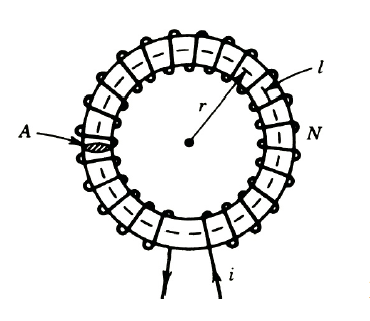
\includegraphics[width=5cm]{figures/toroid.PNG}
            \caption{Toroid}
            \label{fig:toroid}
        \end{figure}

    Consider a toroid (a ring shaped magnetic core), with wires wrapped around the entire circumference as shown in Fig \ref{fig:toroid}.
    When Current flow through the coil, the flux is mostly confined in the core material. The flux outside is called 
    leakage flux and it can usually be neglected. Consider a path at a radius r. The magnetic intensity on this path is H.
   
    
        \begin{align*}
            \oint H\cdot dl = Ni\\
            Hl = Ni\\
            H \cdot 2 \pi r = Ni
        \end{align*}
        where $N\cdot i$ is the magnetomotive force $mmf$.

        \begin{align*}
            Hl = Ni\\
            H = \frac{N}{l}\cdot i\\
            B = \frac{\mu Ni}{l} [Tesla]
        \end{align*}
    
    Assume that all the fluxes are confined in the toroid (no magnetic leakage). The magnetic flux across in the 
    cross section of the toroid is,
        \begin{align*}
            \Phi = \int{BdA}\\
            \Phi = BA[Wb]
        \end{align*}
    where B is the flux density in the core and A is the cross section area of the toroid.
    Let H be the magnetic intensity for this path,
        \begin{align*}
            \Phi &= \frac{\mu Ni}{l} A = \frac{Ni}{l/(\mu A)}\\
            &= \frac{Ni}{R}
        \end{align*}
    where $R$ is the reluctance of the magnetic path, and $\frac{1}{R}$ is called the permeance of the magnetic path.

    \subsection*{Magnetizing Curve}
        \begin{figure}[H]
            \centering
            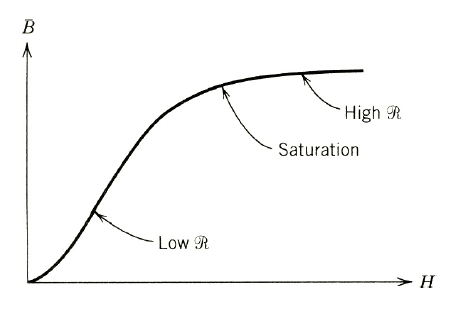
\includegraphics[width=5cm]{figures/magnetizing_curve.PNG}
            \caption{Magnetizing Curve}
            \label{fig:magnetizing_curve}
        \end{figure}


    If the magnetic intensity increased by increasing the current, the flux density in the core changes as shown in Figure \ref{fig:magnetizing_curve}.
    Before saturation, B increases at a rate of $\mu = \mu_{r}\mu_{o}$. After saturation, B increases at a rate of $\mu_{o}$.

    \subsection*{Example}
    \begin{figure}[H]
            \centering
            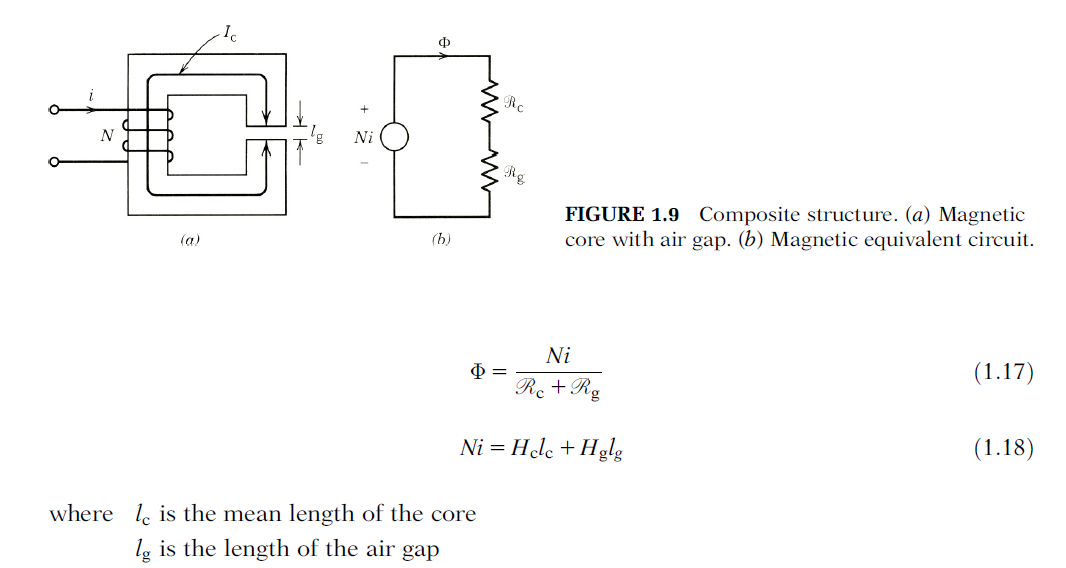
\includegraphics[width=12cm]{figures/magnetic_circuit_example1.PNG}
    \end{figure}

    \subsection*{Faraday's Law}
    A change in flux induces a voltage in the coil and the current flowing through the wire induces a 
    flux that opposes the original flux.
    \begin{equation*}
        e = -N\frac{d\Phi_{original}}{dt}
    \end{equation*}

    \subsection*{Self Inductance}
    \begin{align*}
        &L = \frac{N\Phi}{i}\\
        &Li = N\Phi \rightarrow \text{ flux linkage}
    \end{align*}

    \begin{align*}
        e = \frac{d(N\Phi)}{dt} &= \frac{dLi}{dt}\\
        & = \frac{Ldi}{dt} + \frac{idL}{dt} = \frac{Ldi}{dt}
    \end{align*}

    \begin{equation*}
        L = \frac{N \Phi }{i} = \frac{N^2}{Reluctance}
    \end{equation*}

    \subsection*{Lorentz Force}
    Moving a conductor in a magnetic field induces a current in that conductor.
    If the conductor is perpendicular to the magnetic field,
    \begin{equation*}
        F = i \cdot l \cdot B
    \end{equation*}


    \section*{DC Machine}
    \subsection*{Brushed Motor}

    \begin{figure}[H]
            \centering
            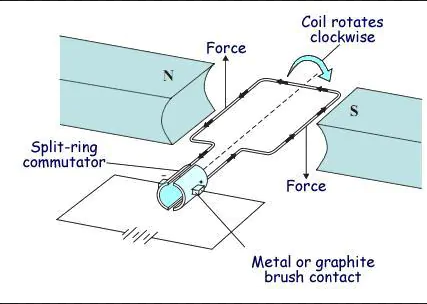
\includegraphics[width=5cm]{figures/brushed_motor.png}
    \end{figure}

    Torque of the motor is given by,
    \begin{align*}
        &T = F \cdot \frac{d}{2} \cdot 2\\
        &T = i\cdot l \cdot B \cdot d \cdot cos \theta \\
        &T = i \cdot A \cdot B \cdot cod \theta = i \Phi cos\theta\\
        &T = k_{T}i_{a} \Phi \text{ where $k_{T}$ is the motor torque constant}
    \end{align*}

    \subsubsection*{Back EMF}
    Since the conductor is moving in the magnetic field, a voltage is induced across the brushes.
    At a speed of $\omega_{m}$, the induced $emf(electromotive force)$ e is,
    \begin{align*}
        &e_{a} = lvB = A B \omega_{m} = \Phi \omega_{m} \\
        &e_{avg} = k_{E}\omega_{m} \Phi
    \end{align*}
    where $n_{a}$ is the number of conductors inside the magnetic field.

    \subsection*{Power}
    \begin{align*}
        P_{e} = P_{m} \rightarrow \text{ideal}\\
        P_{e} = e_{a}i_{a} = k_{e} \Phi \omega_{m} i_{a}\\
        P_{m} = \omega_{m}T_{e} = \omega_{m} k_{T} \Phi i_{a}
    \end{align*}

    \subsection*{Electro-Mechanical Model}
    \begin{figure}[H]
            \centering
            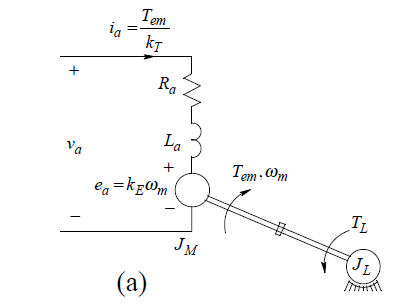
\includegraphics[width=5cm]{figures/elec-mech-model.png}
    \end{figure}
    \begin{align*}
        V = e_{a} + i_{a}R_{a} + L_{a}\frac{di_{a}}{dt}\\
        T_{e} = J_{L}\frac{d\omega_{m}}{dt} + B_{L}\omega_{m} T_{L}
    \end{align*}

    \subsection*{Regenerative Braking}
    While the motor is in steady state, $V>E_{a}$ and $i_{a}$ is positive. If V is decreased while 
    the motor is still moving forward, when $V < E_{a}$, $i_{a}$ is negative, creating a torque that 
    opposes the forward spinning, which decreases the motor speed.

    \subsection*{Generating Magnetic Field}    
    \subsubsection*{Permanent Magnet}
    \begin{align*}
        \Phi = \text{constant}\\
        e_{a} = k_{e} \Phi \omega_{m} = k_{E} \omega_{m}\\
        T_{e} = k_{t} \Phi \omega_{m} = k_{T} \omega_{m}
    \end{align*}

    \subsubsection*{Field Winding}
    \begin{align*}
        \Phi = k_{f}i_{f}\\
        e_{a} = k_{v}k_{f}i_{f} \omega_{m}\\
        T_{e} = k_{t} k_{f} i_{f} i_{a}
    \end{align*}



        

    

    


\end{document}